\documentclass[conference]{IEEEtran}
\IEEEoverridecommandlockouts
% ---------------------------------------------------------------
% Meika: Explainable AI-Based Personal Financial Copilot
% Journal Paper Draft -- Introduction + Literature Survey
% IEEE format (IEEEtran), ready for Overleaf
% ---------------------------------------------------------------
\usepackage{cite}
\usepackage{amsmath,amssymb,amsfonts}
\usepackage{algorithmic}
\usepackage{graphicx}
\graphicspath{{figures/}}
\usepackage{textcomp}
\usepackage{xcolor}
\usepackage[hidelinks]{hyperref}

\def\BibTeX{{\rm B\kern-.05em{\sc i\kern-.025em b}\kern-.08em
    T\kern-.1667em\lower.7ex\hbox{E}\kern-.125emX}}

\begin{document}

\title{MEIKA: An Explainable AI-Based Personal Financial Copilot for\\ Predictive Budgeting, Goal Forecasting, and Financial Risk Analysis}

% ---------------------------------------------------------------
% AUTHOR BLOCK
% ---------------------------------------------------------------
\author{
\IEEEauthorblockN{Doron Linton Prince (23CU0330010), Kannapiran R (23CU0330020), Baskar Adithiya S (23CU0330006)}
\IEEEauthorblockA{Department of Computer Science and Engineering (AI \& ML) \\
Hindustan Institute of Technology and Science \\
Chennai, India}
}

\maketitle

\begin{abstract}
Personal financial management applications are abundant, yet most remain retrospective: they record transactions and render historical summaries without projecting a user's future financial position. Where artificial intelligence is applied, its outputs are typically presented as bare predictions or scores, offering no account of the reasoning that produced them -- a transparency deficit that recent surveys identify as a principal obstacle to trust in financial AI. This paper presents MEIKA, an Explainable AI (XAI)-based personal financial copilot in which explainability is a structural constraint rather than a post-hoc addition. MEIKA computes predictive budgeting indicators -- spending velocity and a projected month-end spend -- directly from live transaction data, and combines them with a category-concentration measure into a deterministic Financial Clarity Score. Every component of that score is emitted as a named \texttt{XAIFactor} object carrying a label, an explanatory detail, and the computed value, so that no figure reaches the user without its own justification. The system is a decoupled monorepo: a Flutter client, a layered FastAPI backend with Pydantic validation and asynchronous SQLAlchemy over a tenant-isolated PostgreSQL schema, and a bounded Gemini reasoning layer restricted to rephrasing already-computed factors. At the Phase-I review the prototype demonstrated three tested REST modules producing a Clarity Score of 91/100 with three live factors over a seeded dataset; the implementation has since been extended with a grounded conversational copilot, a price-comparison module, authentication, and multi-currency display. Explainable goal forecasting and empirical calibration of the score remain the principal items of future work.
\end{abstract}

\begin{IEEEkeywords}
Explainable Artificial Intelligence, Personal Finance Management, Predictive Budgeting, Financial Risk Analysis, Financial Clarity Score, Decision Support Systems, FinTech, FastAPI
\end{IEEEkeywords}

\section{Introduction}

Managing personal finances is one of the most universal, yet persistently difficult, aspects of everyday life. Individuals today manage income and expenditure across a growing number of channels -- bank accounts, digital wallets, credit cards, and subscription services -- generating a volume of transactional data that few tools help them meaningfully interpret \cite{badiger2026spendai}. Numerous budgeting and expense-tracking applications have emerged to address this problem, and empirical reviews of these tools show they are effective at what they were built to do: record what has already happened. Existing systems are repeatedly found to suffer from fragmented financial data, limited real-time insight, and traditional tracking methods that stop short of intelligent, proactive decision-making \cite{deepthi2026aipowered}--\cite{ganta2025multimodule}. Even where machine learning has improved the accuracy of automatic transaction categorization, the underlying decision logic that is exposed to the user typically remains a bare forecast rather than an explanation \cite{deepthi2026aipowered}.

The rapid advancement of Artificial Intelligence (AI), Machine Learning (ML), Explainable AI (XAI), and Large Language Models (LLMs) creates an opportunity to reimagine these tools as genuine financial assistants rather than passive ledgers. Recent prototypes illustrate both the promise and the limits of this shift. Deepthi et al. describe a serverless AI-Powered Finance Management Platform that layers tree-based classifiers, time-series forecasting, and an LLM-based conversational assistant onto a microservices architecture, reporting strong fraud-detection accuracy, yet the paper itself frames explainability as a secondary addition rather than a structural requirement of the system \cite{deepthi2026aipowered}. Ganta et al. propose a multi-module financial assistant integrating fraud detection, credit recommendation, and a document-aware chatbot, and find that existing fintech tools largely operate as isolated modules rather than a single coherent, transparent system \cite{ganta2025multimodule}. At the model layer, independent surveys of large language models in finance converge on the same conclusion: LLMs are increasingly capable of financial reasoning and decision support, but data privacy, bias, and explainability remain the field's most pressing open challenges \cite{nie2024survey}, \cite{khan2025bridging}.

These converging observations motivate the central premise of this project. Rather than adding another predictive feature to a conventional budgeting app, the objective is to make transparency a first-class design constraint: every ``buy,'' ``wait,'' or budget-adjustment recommendation the system produces should be traceable to the specific computed factors -- spending velocity, category drift, projected cash-flow risk -- that generated it, rather than to an opaque model output the user is asked to trust on faith.

Building on this motivation, this paper proposes MEIKA, an Explainable AI-Based Personal Financial Copilot for predictive budgeting, financial-goal forecasting, and financial-risk analysis. MEIKA is intended for students, salaried professionals, freelancers, and families who wish not only to track their spending but to understand and act on it with confidence.

The principal contributions of this work are as follows.

\begin{enumerate}
\item An explainable financial risk-scoring framework in which a bounded Financial Clarity Score is derived from named, auditable factors by a deterministic penalty function, with no trained model and therefore no unauditable inference step.
\item A predictive budgeting mechanism based on spending velocity and month-end projection computed from live transaction data, including an explicit warm-up guard that withholds a projection rather than reporting one drawn from statistically thin data.
\item A traceable XAI representation, the \texttt{XAIFactor} object, carried in the same response schema as the score it justifies, so that a score cannot structurally be transmitted or displayed without its reasoning.
\item A unified architecture combining expense tracking, budget analytics, purchase decision support, and conversational assistance over a single tenant-isolated schema, addressing the fragmentation identified in the reviewed literature.
\item A bounded conversational layer in which the language model may rephrase computed figures but is never granted authority to originate them, together with a deterministic reply path that operates when the model is unavailable.
\end{enumerate}

The remainder of this paper is organized as follows. Section II reviews the literature informing this design and Section III states the resulting research problem. Sections IV and V describe the proposed system and its architecture, Section VI formalizes the methodology, and Section VII reports the implementation. Section VIII presents the prototype evaluation, Section IX positions the system comparatively, and Sections X through XII state its limitations, the planned future work, and the conclusions drawn.

\section{Literature Survey}

This section reviews recent work on AI-driven personal finance platforms, multi-module and risk-aware financial assistants, large language models applied to finance, and the decision-support-systems (DSS) literature that grounds the architectural design of the proposed system. Table~\ref{tab:litsurvey} summarizes the ten papers surveyed, including their methodology, key findings, and the specific limitation or gap each leaves open; the discussion below expands on the entries most relevant to the proposed architecture.

\begin{table*}[!t]
\centering
\caption{Summary of Literature Survey}
\label{tab:litsurvey}
\footnotesize
\renewcommand{\arraystretch}{1.3}
\begin{tabular}{|c|p{2.3cm}|p{4.3cm}|p{3.6cm}|p{3.3cm}|p{3.3cm}|}
\hline
\textbf{S.No} & \textbf{Author \& Year} & \textbf{Paper Title} & \textbf{Method/Technology} & \textbf{Key Finding} & \textbf{Limitation/Gap} \\
\hline
1 & Pathak, 2010 (Base Paper) \cite{pathak2010survey} & A Survey of the Comparison Shopping Agent-Based Decision Support Systems & Survey; 4-component DSS framework (data, models, interfaces, customization) & Provides the DSS framework adopted to structure MEIKA's architecture & E-commerce context, not finance-specific; used only for architectural grounding \\
\hline
2 & Badiger et al., 2026 \cite{badiger2026spendai} & Next.js-Powered AI Platform for Smart Expense Tracking, Budgeting and Insights & Next.js, Prisma, Supabase Postgres + Gemini LLM categorization & 91\% categorization accuracy; $\sim$78\% less manual logging effort & Limited explainability, single-source data, little personalization \\
\hline
3 & Deepthi C G et al., 2026 \cite{deepthi2026aipowered} & AI-Powered Finance Management Platform & XGBoost/RF + ARIMA/LSTM + LLM chat + SHAP (serverless microservices) & 98\% fraud-detection accuracy & Explainability is an add-on to select models, not structural \\
\hline
4 & Kakulapati et al., 2026 \cite{kakulapati2026expensetracker} & AI-Powered Personal Expense Tracker & Django backend, linear regression, NLP, React UI & Effective short-horizon expense prediction \& anomaly ID & No goal forecasting/risk analysis; reasoning not exposed to user \\
\hline
5 & Ganta et al., 2025 \cite{ganta2025multimodule} & An Intelligent Multi-Module Financial Assistant for Personalized Budgeting, Risk Alerts, and Adaptive Investment Advisory & Fraud detection + learning-to-rank credit recommender + document-grounded chatbot & Frames fragmentation as the core weakness of fintech tools & Data sensitivity, explainability, modular scalability unaddressed \\
\hline
6 & Nie et al., 2024 \cite{nie2024survey} & A Survey of Large Language Models for Financial Applications & Survey/taxonomy of LLMs across financial tasks & LLMs improve financial reasoning, planning, real-time tasks & Explainability \& ethics remain the field's most pressing challenges \\
\hline
7 & Khan, Li \& Cao, 2025 \cite{khan2025bridging} & Bridging Finance and AI: A Comprehensive Survey of LLMs in Financial System & Survey; multi-level accuracy/cost/privacy framework & Identifies privacy, bias, explainability as deployment obstacles & Calls for ``more transparent, effective, inclusive financial AI'' \\
\hline
8 & Unde S.P. et al., 2026 \cite{unde2026dashboard} & AI-Based Real-Time Personal Finance Dashboard & Banking-API ingestion + CNN/YOLOv4 OCR + BERT/LSTM + autoencoders + LLM (RAG) advisory & Unifies real-time consolidation, anomaly detection, AI advisory & Most systems isolate tasks; no unified real-time explainable dashboard \\
\hline
9 & Saini et al., 2025 \cite{saini2025aipowered} & AI-Powered Personal Finance Management Applications & Review of ML/NLP/predictive analytics + comparative app analysis (Mint, Cleo, YNAB, etc.) & Broad survey of AI capability across budgeting, investing, literacy & Flags data quality, legacy integration, bias/fairness, transparency gaps \\
\hline
10 & Patil et al., 2026 \cite{patil2026nexus} & Nexus Finance: AI-Powered Financial Goal Planner for Personalized Budgeting and Investment & K-Means clustering + Random Forest, with nudge-theory-based prompting & Reports 91\%/88\% accuracy for financial health scoring and user segmentation & No explainability treatment; time-series forecasting and bank integration left as future work \\
\hline
\end{tabular}
\end{table*}

\subsection{AI-Driven Personal Finance Management Platforms}

Badiger et al. present Spend AI, a full-stack personal finance platform built on Next.js, Prisma ORM, and Supabase PostgreSQL that integrates Google's Gemini LLM for automated transaction categorization, anomaly detection, and natural-language financial insights \cite{badiger2026spendai}. Evaluated against India's UPI-driven digital payment ecosystem, the system reports over 91\% transaction-categorization accuracy and an approximately 78\% reduction in manual expense-logging effort. The authors explicitly identify limited explainability, single-source data dependency, and a lack of personalization as gaps their architecture only partially closes.

Unde et al. similarly propose an AI-Based Real-Time Personal Finance Dashboard that consolidates fragmented financial data through banking-API ingestion, CNN/YOLOv4-based OCR for receipt digitization, BERT/LSTM models for categorization and savings forecasting, and autoencoder-based anomaly detection, paired with an LLM-driven advisory chatbot \cite{unde2026dashboard}. The authors' own review of contemporary systems concludes that most contemporary tools address isolated tasks -- either receipt scanning or budgeting -- with a persistent lack of a unified, real-time dashboard that concurrently integrates visual recognition, anomaly detection, and cross-platform data consolidation. Saini et al. take a broader view, surveying AI's role across categorization, budgeting, robo-advisory, and financial-literacy tools (e.g., Mint, Cleo, YNAB, Betterment) and concluding that, despite rapid capability growth, data quality, legacy-system integration, algorithmic fairness, and -- again -- transparency in AI-generated recommendations remain open, field-wide challenges \cite{saini2025aipowered}.

Deepthi et al. describe a serverless, microservices-based AI-Powered Finance Management Platform combining XGBoost and Random Forest classifiers for transaction categorization and fraud detection, ARIMA/LSTM time-series models for budgeting and forecasting, and an LLM (Gemini/GPT-4) for conversational financial advice, with SHAP used to make selected predictions interpretable \cite{deepthi2026aipowered}. Reported fraud-detection accuracy reaches 98\%, but explainability is treated as an add-on technique applied to specific models rather than as a property enforced across every recommendation the system produces.

Kakulapati et al.'s AI-Powered Personal Expense Tracker uses a Django backend and a linear-regression model to evaluate historical expenditures and predict forthcoming spending patterns, recommending expenditure categories via natural-language processing and delivering results through a React interface \cite{kakulapati2026expensetracker}. While effective for short-horizon expense prediction and anomaly identification, the system does not address longer-term goal forecasting or structured risk analysis, and its predictive reasoning is not exposed to the end user in an explainable form.

Patil et al. approach the problem from the goal-planning direction, proposing Nexus Finance, an AI-powered financial goal planner that applies K-Means clustering for user segmentation and a Random Forest classifier for financial health scoring, reinforced by nudge-theory-based behavioural prompting \cite{patil2026nexus}. The reported segmentation and scoring accuracies are strong, and the work is the closest of those surveyed to the goal-forecasting objective of the present system. It is also instructive in what it defers: time-series forecasting and live bank integration are left as future work, and the health score itself is delivered as a classifier output without a factor-level account of what produced it. The gap this leaves -- goal-oriented financial guidance that is simultaneously forward-looking and explainable -- is precisely the one the proposed system targets.

\subsection{Multi-Module and Risk-Aware Financial Assistants}

Ganta et al. propose a Personalized Financial Assistant that unifies fraud detection, a learning-to-rank credit-card recommender, and a document-grounded conversational chatbot within a single modular pipeline, using category-aware document embeddings and semantic user profiling to personalize output \cite{ganta2025multimodule}. The work is notable for explicitly framing fragmentation -- rather than raw predictive accuracy -- as the central weakness of the fintech landscape: existing tools solve narrow subdomains such as expense tracking, credit ranking, or robo-advice in isolation, with little integration or shared context between them, and challenges such as data sensitivity, explainability, and modular scalability remain under-addressed.

\subsection{Large Language Models in Financial Applications}

Nie et al. provide a comprehensive survey of large language models applied to finance, cataloguing applications across linguistic tasks, sentiment analysis, financial time-series analysis, financial reasoning, and agent-based modelling \cite{nie2024survey}. The survey concludes that while LLMs demonstrably improve contextual understanding of financial data and support planning, recommendation, and real-time reasoning tasks, ethical issues -- with explainability foremost among them -- remain among the field's most pressing open challenges.

Khan, Li, and Cao similarly survey LLMs across the broader financial system, presenting a taxonomy spanning text processing, forecasting, and question-answering tasks and proposing a multi-level framework for balancing model accuracy, computational cost, and data privacy \cite{khan2025bridging}. The survey identifies data privacy, bias, and explainability as the primary deployment obstacles to trustworthy financial AI, and calls explicitly for ``more transparent, effective, and inclusive financial AI'' as a future research direction. Read together, these two surveys support the central design premise of the present work: an LLM-based financial copilot is only as trustworthy as the reasoning it is willing to expose.

\subsection{Decision Support Systems Foundations}

Beyond finance-specific AI literature, this project draws its architectural grounding from Pathak's survey of comparison-shopping-agent-based decision support systems (DSS), adopted as the base paper for this work \cite{pathak2010survey}. Pathak characterizes a comprehensive DSS as requiring four components -- data, models, interfaces, and user-specific customization -- and uses this framework to synthesize contemporary research on web-based shopping agents. Although developed in the context of e-commerce price comparison rather than personal finance, this four-component framework maps directly onto the proposed system's own architecture: a data layer (transaction and account ingestion), a models layer (predictive budgeting, risk, and Financial Clarity Score computation), an interface layer (the client application and conversational UI), and a customization layer (per-user, tenant-scoped personalization). This framework is used in the present work to structure the system architecture and to justify why explainability and personalization must be treated as core architectural components rather than optional features.

\subsection{Research Gap}

Across this body of work, a consistent pattern emerges. Systems that achieve strong predictive or classification performance -- Badiger et al.'s 91\% categorization accuracy \cite{badiger2026spendai}; Deepthi et al.'s 98\% fraud-detection accuracy \cite{deepthi2026aipowered} -- treat explainability as an auxiliary feature rather than a structural constraint on every output. Systems that integrate multiple financial functions into a single assistant \cite{ganta2025multimodule} do not extend that integration to genuine long-term goal forecasting or a formally justified decision-support architecture, and the one surveyed system built explicitly around goal planning \cite{patil2026nexus} defers both time-series forecasting and any factor-level account of the scores it produces. And the LLM-in-finance surveys \cite{nie2024survey}, \cite{khan2025bridging} confirm, at a field level, that explainability and trust remain unresolved even as underlying model capability continues to grow. No reviewed system combines predictive budgeting, financial-goal forecasting, financial-risk analysis, and a conversational interface within a single platform in which every recommendation is required to carry its own computed justification, grounded in an explicit decision-support framework \cite{pathak2010survey}. This is the gap the proposed system, MEIKA, is designed to address.


\section{Problem Statement and Research Gap}

The systems reviewed in Section II share a structural characteristic: they are, in the main, systems of record rather than systems of foresight. A conventional personal-finance application ingests or accepts transactions, normalizes them into categories, and renders the result as a historical summary. The user learns what has already happened. Where predictive components are present, they are typically confined to short-horizon categorization or expenditure forecasting \cite{kakulapati2026expensetracker}, \cite{badiger2026spendai}, and where those predictions are surfaced, they are surfaced as bare outputs. The user is shown a number and asked to accept it.

This produces a compound problem. First, financial difficulty is detected only after it has materialized: a user discovers an overspend at the end of the month, when no corrective action remains available. Second, the artificial-intelligence components introduced to address this are themselves opaque, so a user who is warned has no basis on which to evaluate the warning. Saini et al. document this directly, observing that user trust increases as financial AI shifts away from black-boxed operation toward transparent and explanative behaviour \cite{saini2025aipowered}; Nie et al. and Khan et al. reach the same conclusion at the level of the underlying models \cite{nie2024survey}, \cite{khan2025bridging}. Third, the functions a user actually needs -- tracking, projection, risk detection, goal planning, and purchase decision support -- are distributed across single-purpose tools that share neither a schema nor a context, a fragmentation Ganta et al. identify as the central weakness of the contemporary fintech landscape \cite{ganta2025multimodule}.

The central research problem addressed by this work may therefore be stated as follows:

\begin{quote}
\emph{How can a personal financial-management system deliver predictive insight and proactive financial-risk analysis while guaranteeing that every score, warning, or recommendation it produces remains understandable and traceable to identifiable, auditable financial factors?}
\end{quote}

The emphasis on \emph{guaranteeing} is deliberate. An explanation produced by a secondary interpretability technique applied to a subset of model outputs, as in the SHAP layer of Deepthi et al. \cite{deepthi2026aipowered}, is an explanation the architecture permits but does not require. The position taken here is that explainability must be enforced by construction: if a value cannot be decomposed into named contributing factors, it is not shown. Table~\ref{tab:researchgap} summarizes the specific gaps identified across the surveyed literature and the corresponding design response in the proposed system.

\begin{table*}[!t]
\centering
\caption{Research Gaps and the Corresponding MEIKA Design Response}
\label{tab:researchgap}
\footnotesize
\renewcommand{\arraystretch}{1.35}
\begin{tabular}{|p{4.2cm}|p{6.3cm}|p{6.6cm}|}
\hline
\textbf{Research Gap} & \textbf{Existing Limitation} & \textbf{MEIKA Approach} \\
\hline
G1. Predictions delivered without reasoning & Predictive outputs are presented as bare figures; the contributing factors are not exposed to the user \cite{kakulapati2026expensetracker}, \cite{deepthi2026aipowered} & Every score is decomposed into named \texttt{XAIFactor} objects (label, detail, value) rendered alongside the score in the client \\
\hline
G2. Black-box models erode user trust & Trained models yield outputs that cannot be audited by the user, reducing willingness to act on advice \cite{saini2025aipowered} & The Financial Clarity Score is computed by a deterministic, rule-based penalty function, not a trained model; identical inputs always yield an identical, inspectable score \\
\hline
G3. Fragmented, single-purpose tooling & Tracking, budgeting, risk alerting, and purchase support are split across unintegrated applications \cite{ganta2025multimodule}, \cite{unde2026dashboard} & One tenant-isolated PostgreSQL schema and a single service layer span expense capture, budget analytics, price comparison, and conversational assistance \\
\hline
G4. Retrospective rather than forward-looking analysis & Systems report historical spend; conceptual surveys propose forecasting without shipping it \cite{nie2024survey}, \cite{khan2025bridging} & Spending velocity and month-end projection are computed from live transaction rows on every dashboard request, with a warm-up guard that suppresses projections drawn from statistically thin data \\
\hline
G5. Absence of explainable goal forecasting & Goal planning is either absent or delivered without interpretable reasoning; forecasting is deferred to future work \cite{patil2026nexus} & Goal forecasting is scoped as a planned module held to the same construction-time explainability constraint as the Clarity Score (see Section XI) \\
\hline
\end{tabular}
\end{table*}

\section{Proposed System}

MEIKA is proposed as an explainable AI-based personal financial copilot: an application that not only records expenditure but projects its consequences and justifies every projection it makes. The system is organized as a set of cooperating modules, described below. Consistent with the reporting discipline adopted throughout this paper, each module is annotated with its verified implementation status.

\subsection{Expense Management (Implemented)}

Users record expenditure through the Flutter client, either by manual entry or by the development seeding utility used for demonstration. Each expense carries a title, a category drawn from a fixed eight-member enumeration, an amount, an optional store reference, a transit cost and mode, an occurrence date, and the owning \texttt{user\_id}. Requests are validated against Pydantic schemas at the API boundary and persisted to PostgreSQL through asynchronous SQLAlchemy. A full create, read, update, and delete surface is exposed over REST.

\subsection{Predictive Budgeting (Implemented)}

From the transactions recorded in the current calendar month, the system derives a spending velocity -- expenditure per elapsed day -- and extrapolates it across the full month to obtain a projected month-end spend, together with any projected overage against the user's configured monthly budget. The projection is deliberately suppressed when fewer than seven days of data are available in the month, on the grounds that a single ordinary purchase early in a month produces a projection that swings wildly and would convey false confidence.

\subsection{Financial Clarity Score (Implemented)}

The Clarity Score is a bounded integer in $[0, 100]$ expressing the user's current financial risk posture, accompanied by a categorical risk level. It is computed deterministically by subtracting penalties contributed by each analysed factor from a nominal maximum, as formalized in Section VI. It is explicitly \emph{not} the output of a trained model: no training data, no learned weights, and no inference step are involved, which is precisely what makes the score auditable line by line.

\subsection{Explainability Layer (Implemented)}

Each factor contributing to the Clarity Score is emitted as a named \texttt{XAIFactor} object with three fields: a \texttt{label} naming the condition detected, a \texttt{detail} string stating in natural language the quantities that produced it, and a numeric \texttt{value} carrying the computed magnitude. The factor list is returned in the same API response as the score itself and is rendered adjacent to it in the client. A score is therefore never transmitted or displayed without its own justification; the two are structurally inseparable in the response schema.

\subsection{Financial Risk Analysis (Implemented)}

Risk is assessed along three concurrent axes: spending pace relative to an even distribution of the monthly budget, projected month-end outcome relative to that budget, and concentration of expenditure within a single category. These correspond to the three live factors demonstrated at the Phase-I review -- pace, projection, and concentration -- and each contributes both a penalty to the score and an explanatory factor to the response.

\subsection{Goal Forecasting (Planned)}

Goal forecasting -- projecting whether a defined savings or spending target remains achievable given the observed spend trend -- is a stated objective of the project and is \emph{not} implemented at the time of writing. A source-level inspection of the backend and client confirms that no goal model, service, or endpoint currently exists. It is described here as a planned extension only, and is treated as such throughout this paper.

\subsection{Conversational Copilot (Implemented, with a Bounded and Partially Unvalidated Model Path)}

The conversational layer is exposed over a WebSocket endpoint and is grounded by construction: replies are assembled from the same computed Clarity Score factors and price-comparison results that the dashboard uses, and chat history is persisted. Three distinct states must be separated for accuracy. The transport, grounding pipeline, history persistence, and deterministic reply path are implemented and covered by automated tests. The live Gemini generation path is implemented and wrapped such that any failure degrades to the deterministic path, but it has not been validated against a live API key. The model's role is bounded by design: it may rephrase already-computed figures conversationally, but it is not a source of financial figures and cannot introduce values the deterministic layer did not compute.

\subsection{Price-Finder and True Economic Cost (Implemented)}

A supporting module compares the true economic cost of a prospective purchase -- sticker price plus the transit cost of acquiring it -- across retailers, returning a computed rather than asserted recommendation. It operates over a seeded catalog and, where an external search key is configured, over live retail search results, falling back to the seeded catalog when the external service is unavailable. Consistent with the explainability constraint, a price trend is reported as \texttt{insufficient\_data} for a listing observed only once, rather than asserting a direction the available data does not support.

\section{System Architecture}

MEIKA is implemented as a decoupled monorepo comprising a Flutter client and a layered FastAPI backend over PostgreSQL. The architecture is shown in Fig.~\ref{fig:architecture} and follows the four-component decision-support structure adopted from Pathak \cite{pathak2010survey}: a data layer, a models layer, an interface layer, and a per-user customization layer.

\begin{figure*}[!t]
\centering
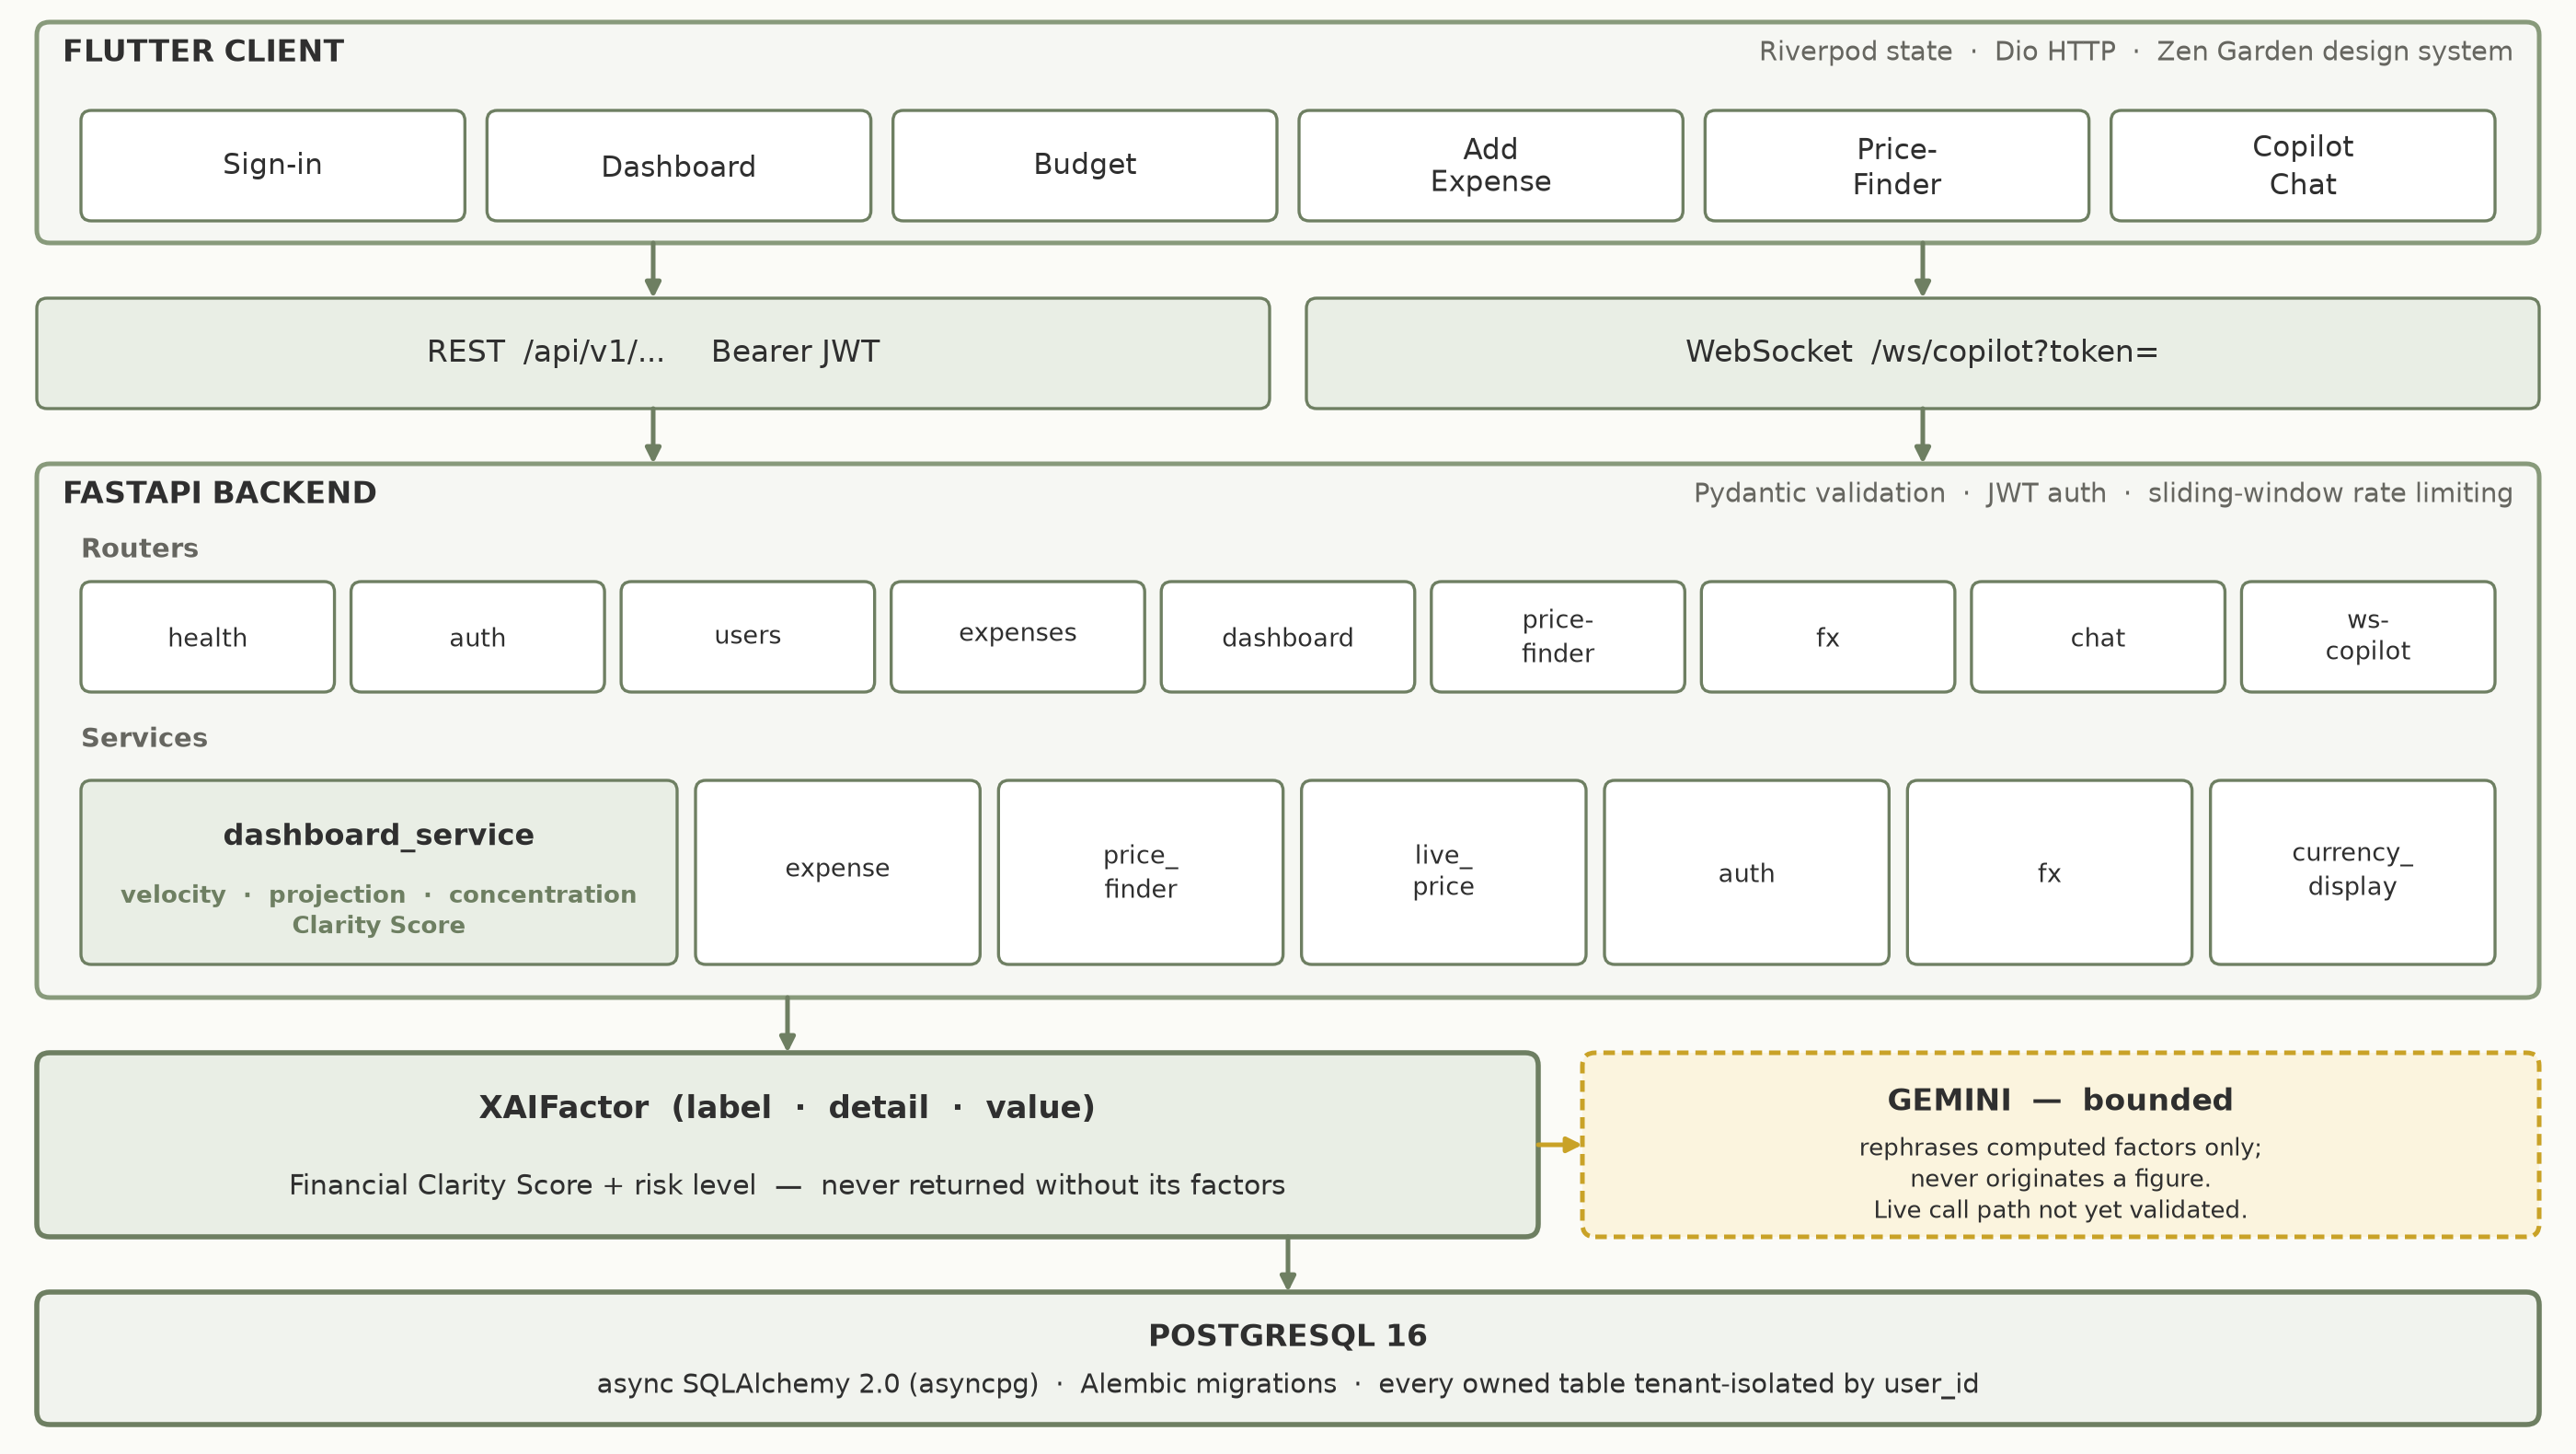
\includegraphics[width=\textwidth]{fig1_architecture.png}
\caption{Overall MEIKA system architecture: Flutter client, layered FastAPI backend, PostgreSQL persistence, and the bounded Gemini reasoning layer. Every computed score leaves the service layer accompanied by the \texttt{XAIFactor} objects that produced it.}
\label{fig:architecture}
\end{figure*}

Requests originate in the Flutter client, where Riverpod manages application state and Dio performs HTTP transport. They arrive at the FastAPI application, which resolves the caller's identity from a signed JSON Web Token, applies rate limiting, and validates the request body against a Pydantic schema. Routing is thin by design: routers delegate to a service layer, and it is in that layer -- principally \texttt{dashboard\_service} -- that all financial computation occurs. The service layer reads from PostgreSQL through asynchronous SQLAlchemy sessions, computes the predictive indicators, assembles the explanatory factors, derives the Clarity Score, and returns a composite response object carrying data and explanation together. Conversational traffic follows the same path but enters over a WebSocket, with the token supplied as a query parameter because a browser WebSocket handshake cannot carry a custom authorization header.

Tenant isolation is enforced structurally rather than by convention. Every user-owned table carries a \texttt{user\_id} column from the initial migration onward, and every query against user-owned data is scoped through it. The identifier is in all cases derived from the verified token rather than accepted from the request body, so a caller cannot address another tenant's rows by manipulating a parameter. One deliberate exception exists: the shared product catalog is not user-owned data and remains searchable without authentication, with a token, where present, used only to personalize currency display. The schema is version-controlled through Alembic migrations, of which three are present at the time of writing. Table~\ref{tab:techstack} lists the technology stack.

\begin{table}[!t]
\centering
\caption{Technology Stack}
\label{tab:techstack}
\footnotesize
\renewcommand{\arraystretch}{1.3}
\begin{tabular}{|p{2.4cm}|p{5.3cm}|}
\hline
\textbf{Layer} & \textbf{Technologies} \\
\hline
Languages & Python 3.12, Dart \\
\hline
Client & Flutter, Riverpod (state), Dio (HTTP) \\
\hline
Backend framework & FastAPI, Pydantic, Uvicorn (ASGI) \\
\hline
Persistence & PostgreSQL 16, SQLAlchemy 2.0 (async), Alembic, asyncpg \\
\hline
Security & JWT (PyJWT), bcrypt password hashing, in-process sliding-window rate limiting \\
\hline
XAI layer & Deterministic factor-based scoring engine emitting \texttt{XAIFactor} objects \\
\hline
Language model & Gemini, bounded to rephrasing computed factors (live call path not yet validated) \\
\hline
Testing & pytest with an HTTP test client \\
\hline
Environment & Standard developer workstation; no GPU and no model training required \\
\hline
\end{tabular}
\end{table}

A property of this architecture worth stating explicitly is that it requires no training infrastructure. Because the risk model is deterministic, the system has no training corpus, no periodic retraining cycle, and no accuracy figure that can silently drift as a learned distribution ages. This is a deliberate trade: the system forgoes the pattern-discovery capability of a learned model in exchange for outputs that are reproducible and auditable by construction.

\section{Methodology}

The end-to-end workflow proceeds in seven steps, illustrated in Fig.~\ref{fig:workflow}. Steps 1 through 6 are implemented; step 7 is implemented in its transport and grounding but retains an unvalidated model path, as qualified below.

\begin{figure}[!t]
\centering
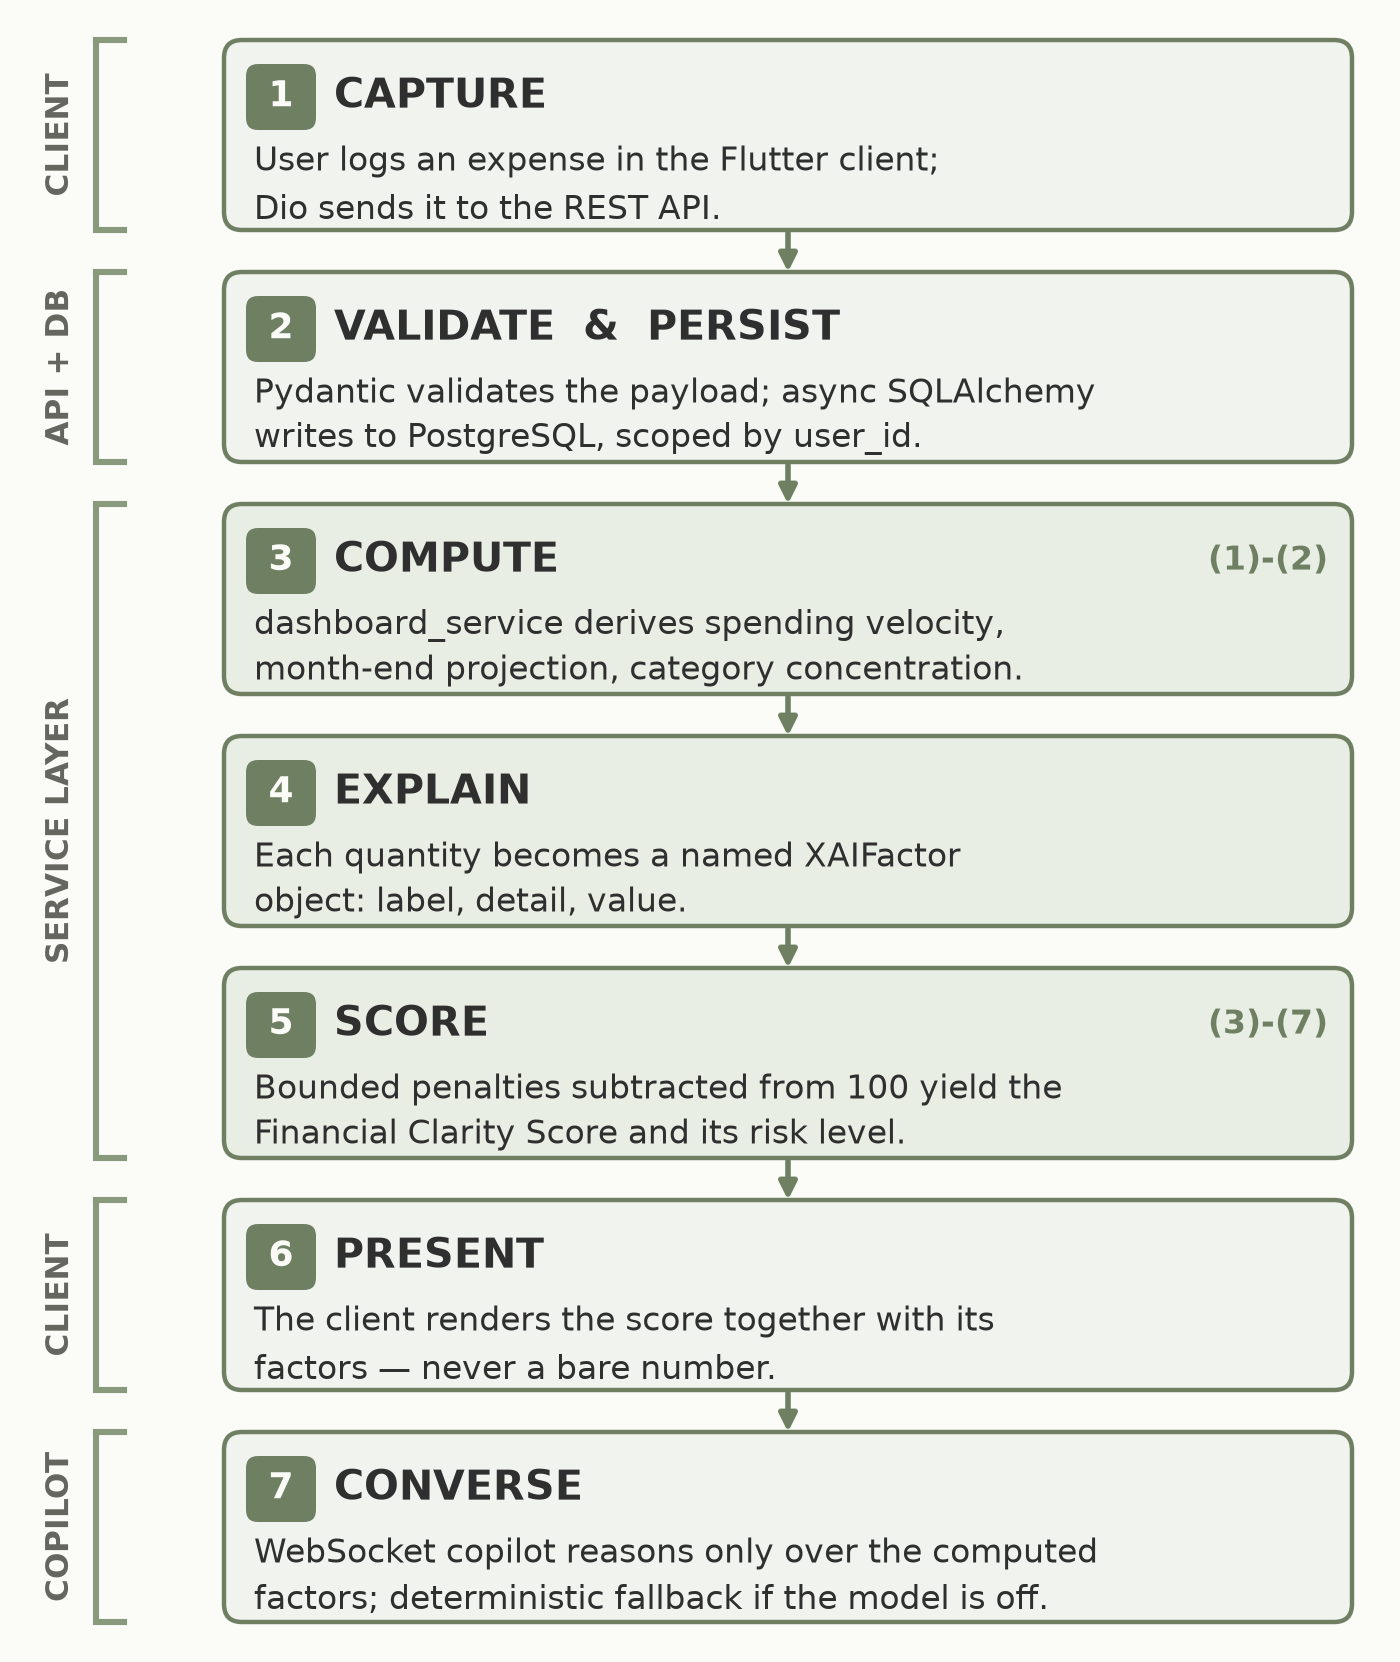
\includegraphics[width=\columnwidth]{fig2_workflow.png}
\caption{End-to-end methodology workflow from expense capture to explained presentation.}
\label{fig:workflow}
\end{figure}

\subsection{Step 1: Capture}

The user records an expense in the Flutter client. The client serializes the entry and transmits it to the REST API over HTTP via Dio, attaching the bearer token issued at sign-in.

\subsection{Step 2: Validate and Persist}

FastAPI validates the payload against a Pydantic schema, rejecting malformed categories, negative amounts, and absent required fields at the boundary before any database interaction occurs. The validated entity is written to PostgreSQL through an asynchronous SQLAlchemy session, stamped with the \texttt{user\_id} resolved from the verified token.

\subsection{Step 3: Compute}

On each dashboard request, the service layer loads the caller's expenses for the current calendar month and derives the predictive indicators. Let $d$ denote the number of elapsed days in the month, $D$ the total days in that month, $B$ the configured monthly budget, and $S$ the total expenditure recorded month-to-date, where each expense contributes its amount plus its associated transit cost. Spending velocity is the mean daily expenditure over the elapsed period:

\begin{equation}
v = \frac{S}{d}
\end{equation}

Projected month-end expenditure extrapolates that velocity across the full month, and projected overage is the non-negative excess of that projection over the budget:

\begin{equation}
P = v \cdot D, \qquad O = \max(0,\; P - B)
\end{equation}

Equation (2) is evaluated only when $d \geq d_{\min}$, with $d_{\min} = 7$ in the current implementation. Below that threshold the projection is withheld and replaced by an explanatory factor stating why, rather than being reported with unwarranted confidence.

\subsection{Step 4: Explain}

Each computed quantity is assembled into a named \texttt{XAIFactor} object $f = \langle \text{label}, \text{detail}, \text{value} \rangle$. The factors are constructed in the same function that computes the penalties, so a factor and the penalty it justifies cannot diverge: there is no separate explanation-generation pass that could describe something other than what was computed.

\subsection{Step 5: Score}

The Financial Clarity Score is obtained by subtracting bounded penalties from a nominal maximum of 100. Three penalties are defined. Let $E = B \cdot d / D$ be the expenditure expected by day $d$ under an even distribution of the budget, let $r = S/E$ be the resulting pace ratio, and let $c$ be the share of month-to-date expenditure falling in the largest single category. A warm-up coefficient dampens the sample-sensitive penalties early in the month:

\begin{equation}
w = \min\!\left(1,\; \frac{d}{d_{\min}}\right)
\end{equation}

The pace, projection, and concentration penalties are then

\begin{align}
\Pi_{\text{pace}} &= \min\big(35,\; \max(0,\, (r - 1)\cdot 35)\big) \cdot w \\
\Pi_{\text{proj}} &= \min\!\left(40,\; \frac{O}{B}\cdot 40\right) \\
\Pi_{\text{conc}} &= \min\big(15,\; \max(0,\, (c - 0.4)\cdot 25)\big) \cdot w
\end{align}

and the score is the clamped, rounded complement of their sum:

\begin{equation}
\mathrm{CS} = \mathrm{clamp}_{[0,100]}\Big(\big\lfloor 100 - (\Pi_{\text{pace}} + \Pi_{\text{proj}} + \Pi_{\text{conc}}) \big\rceil\Big)
\end{equation}

The score maps to a categorical risk level: \emph{low} for $\mathrm{CS} \geq 70$, \emph{moderate} for $40 \leq \mathrm{CS} < 70$, and \emph{high} below 40. Equations (1) through (7) reflect the current implementation in \texttt{dashboard\_service.py} rather than a conceptual formulation; the constants 35, 40, 25, and 15 are design parameters chosen to weight the three axes, and are candidates for empirical calibration once a larger dataset is available (Section X).

The resulting decomposition is summarized in Fig.~\ref{fig:xaimodel}. The structure of (4) through (6) is what makes the score explainable in the sense claimed here. Each penalty is a function of exactly one named, independently observable quantity, so the contribution of each factor to the final score can be stated, checked, and if necessary disputed by the user. Concentration, in particular, is interpreted as the degree to which expenditure is concentrated within a small number of categories; the implementation penalizes only the share above a $40\%$ tolerance, on the reasoning that some concentration is normal and only pronounced concentration signals fragility.

\begin{figure}[!t]
\centering
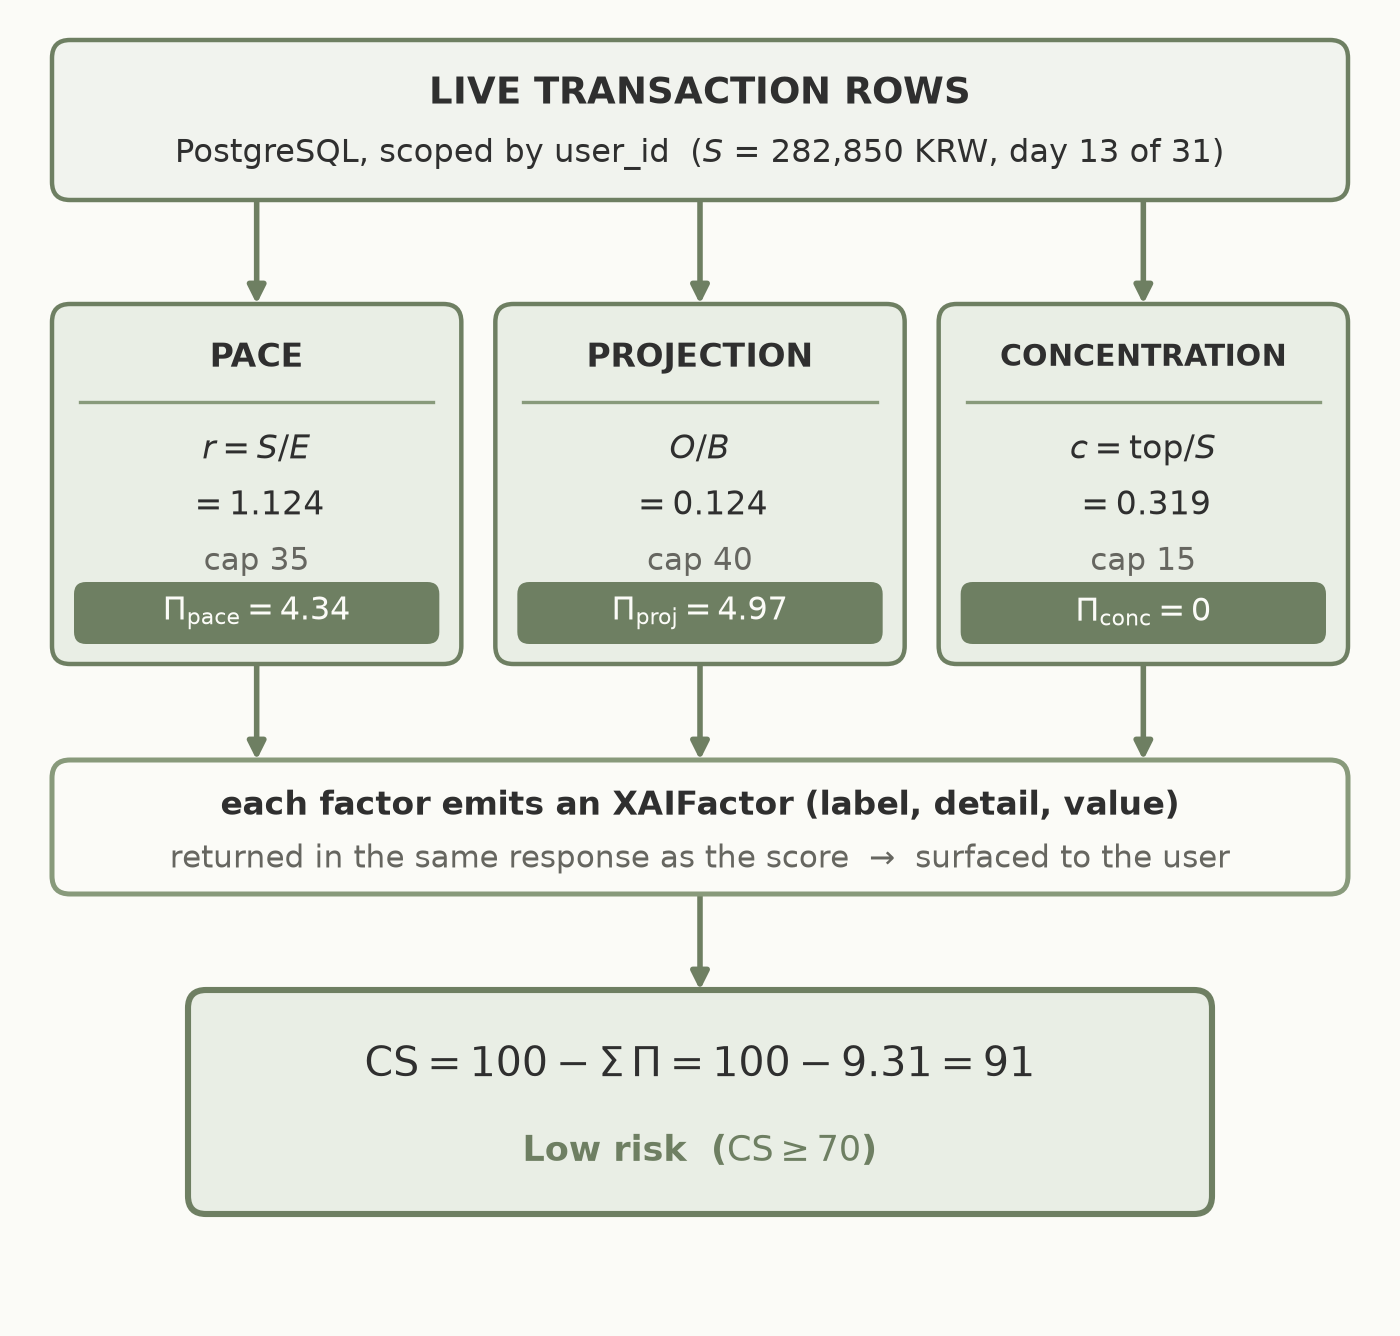
\includegraphics[width=\columnwidth]{fig3_clarity_model.png}
\caption{Decomposition of the Financial Clarity Score into named, auditable factors, shown with the Phase-I demonstration values of Section VIII-E. The penalty caps (35, 40, 15) are fixed design parameters; the quantities and resulting penalties vary with the user's data.}
\label{fig:xaimodel}
\end{figure}

\subsection{Step 6: Present}

The client renders the score together with its factor list. The Budget screen additionally derives a cash-flow runway on the client from the values returned by the API, dividing the remaining budget by the spending velocity to obtain the number of days the budget will last at the current pace and the calendar date on which it would be exhausted. This runway is client-side arithmetic over server-computed inputs, not a separately modelled server-side forecast.

\subsection{Step 7: Conversational Assistance}

A conversational request over the WebSocket triggers the same computation path. The resulting factors form the grounding context for the reply, and the reply is returned together with the factors that justify it. Where the language-model path is unavailable or unconfigured, a deterministic reply constructed directly from those factors is returned instead. The model is never given authority to originate a financial figure.

\section{Implementation}

This section reports the implementation as verified against the source repository at the time of writing. Where a claim is specific to the Phase-I demonstration of 14 August 2026, it is identified as such.

\subsection{Backend}

The backend is a FastAPI application organized into routers, a service layer, schemas, and models. Nine routers expose fourteen REST endpoints together with one WebSocket endpoint, covering health, authentication, users, expenses, dashboard analytics, price comparison, foreign-exchange rates, chat history, and the copilot socket. All request and response bodies are typed through Pydantic schemas. Database access is uniformly asynchronous, using SQLAlchemy 2.0 with asyncpg.

\subsection{Database}

PostgreSQL 16 holds all persistent state. Every user-owned table carries a \texttt{user\_id} foreign key established in the initial migration, and the schema has since evolved through two further Alembic revisions, three in total at the time of writing. At the Phase-I demonstration two migrations had been applied.

\subsection{Frontend}

The Flutter client implements six screens: sign-in, dashboard, budget, add-expense, price-finder, and copilot chat. State is managed with Riverpod and HTTP transport handled by Dio. The dashboard renders the Clarity Score with its factor list; the budget screen renders the cash-flow outlook and expense history; the copilot screen renders chat turns with an expandable panel exposing the computed factors behind each assistant reply.

\subsection{Explainability}

The \texttt{XAIFactor} type is defined once in the shared schema module and reused by the dashboard, price-finder, and copilot response models, so a single definition of "explanation" applies across every surface that produces one. The Clarity Score response cannot be constructed without a factor list, which is what enforces the explainability constraint at the type level rather than by developer discipline.

\subsection{Security}

Authentication is by signed JSON Web Token, with bcrypt password hashing; the interim header-based user identification used during early development has been removed. An in-process sliding-window rate limiter applies a general per-minute request budget and a stricter budget on authentication routes. As documented in the project repository, this constitutes an MVP security baseline rather than a completed security review: there is no refresh-token or revocation flow, no brute-force lockout beyond the rate limit, no transport-security enforcement at the application layer, and the client holds its token in memory only. The rate limiter is per-process and would require a shared store before running multiple workers.

\subsection{Testing}

The test suite comprises eleven pytest modules covering health, authentication, users, expenses, dashboard analytics, price comparison, live price search, foreign exchange, and chat. At the Phase-I demonstration, nine of eleven automated tests passed. The suite has since grown substantially; a full current pass rate is not reported here because executing the complete suite requires a provisioned PostgreSQL instance, which was unavailable in the environment used to prepare this manuscript, and reporting a partial run as a headline figure would misrepresent it. External-service tests are constructed so that they never consume live API quota, using a fixture that disables the external search key and a mocked HTTP client to verify parsing logic.

Table~\ref{tab:status} summarizes the verified status of each module, contrasting the position at the Phase-I review with the position at the time of writing.

\begin{table}[!t]
\centering
\caption{Prototype Implementation Status}
\label{tab:status}
\footnotesize
\renewcommand{\arraystretch}{1.3}
\begin{tabular}{|p{3.6cm}|p{2.0cm}|p{1.6cm}|}
\hline
\textbf{Module} & \textbf{At Phase-I Review} & \textbf{At Time of Writing} \\
\hline
Project scaffold & Implemented & Implemented \\
\hline
Schema, models, migrations & Implemented & Implemented \\
\hline
Velocity, projection, Clarity Score & Implemented & Implemented \\
\hline
Client design system & Implemented & Implemented \\
\hline
Dashboard and budget UI & Partial & Implemented \\
\hline
Price-Finder engine & Partial & Implemented \\
\hline
Copilot WebSocket & Not started & Implemented \\
\hline
Copilot chat UI & Not started & Implemented \\
\hline
JWT auth, rate limiting & Not started & Implemented (MVP baseline) \\
\hline
Live Gemini call path & Not started & Implemented, not validated \\
\hline
Goal forecasting & Not started & Not started \\
\hline
\end{tabular}
\end{table}

\section{Results and Discussion}

The evaluation reported here is a functional and architectural evaluation of a working prototype. It is explicitly \emph{not} a statistical evaluation of predictive accuracy, and no such claim is made. The system contains no trained model, so accuracy, precision, recall, and error metrics such as RMSE or MAPE are not defined quantities for the components currently implemented; reporting them would be meaningless rather than merely premature.

\subsection{Functional Evaluation}

The prototype was exercised end to end against live data. Table~\ref{tab:functional} records the observed outcome for each stage of the workflow defined in Section VI.

\begin{table}[!t]
\centering
\caption{Prototype Functional Evaluation}
\label{tab:functional}
\footnotesize
\renewcommand{\arraystretch}{1.3}
\begin{tabular}{|p{3.5cm}|p{4.2cm}|}
\hline
\textbf{Capability} & \textbf{Observed Outcome} \\
\hline
Accepts expense data & Verified -- entries accepted via client and REST API \\
\hline
Validates requests & Verified -- malformed payloads rejected at the Pydantic boundary \\
\hline
Persists data & Verified -- rows written to PostgreSQL, scoped by \texttt{user\_id} \\
\hline
Computes predictive indicators & Verified -- velocity and month-end projection computed from live rows \\
\hline
Generates XAI factors & Verified -- three named factors returned (pace, projection, concentration) \\
\hline
Produces a Clarity Score & Verified -- deterministic score with categorical risk level \\
\hline
Displays score with reasoning & Verified -- score and factor list rendered together in the client \\
\hline
Suppresses thin projections & Verified -- projection withheld below seven days of data, with a stated reason \\
\hline
\end{tabular}
\end{table}

\subsection{Explainability Evaluation}

The distinguishing property of the system is best assessed structurally rather than numerically. In a conventional pipeline, a score is produced by a model and an explanation, if offered at all, is reconstructed afterwards by a separate interpretability technique applied to that model. Two failure modes follow: the explanation may be unavailable for some outputs, and it is at best an approximation of the model's actual reasoning. In MEIKA, the penalty and the factor that describes it are constructed in the same operation, from the same quantities. The explanation is therefore not an approximation of the computation; it is a restatement of it. The practical consequence, observable in the demonstrated output, is that a user seeing a score of 91 can also see that no pace penalty was incurred because expenditure stood below the even-pace expectation, that the projection remained within budget, and what share of spending the largest category represented.

This structural guarantee is bounded in one important respect. It applies to values the deterministic layer computes. It does not extend to the language model's phrasing of those values, which is constrained by prompt construction and by the deterministic fallback path, but is not itself formally verified.

\subsection{Prototype Testing}

At the Phase-I demonstration, nine of eleven automated tests passed, two Alembic migrations had been applied to a live PostgreSQL schema, and three REST modules -- health, expenses, and dashboard -- were exercised against real data. The two failing tests at that milestone corresponded to modules still under construction at that date.

\subsection{Demonstration Scenario (Phase-I Review, 14 August 2026)}

The Phase-I review demonstrated the system against a seeded dataset of seven transactions distributed across six categories. The dashboard returned a Financial Clarity Score of 91 out of 100, classified as low risk, accompanied by three live factors covering spending pace, month-end projection, and category concentration. The Budget screen reported a cash-flow outlook indicating that, at the observed spending pace, the monthly budget would last until 27 August. Both screens are shown in Fig.~\ref{fig:screens}.

Two qualifications are essential to reading these figures correctly. First, a seven-transaction dataset is a functional demonstration, not a sample from which any statistical inference may be drawn; the figures demonstrate that the pipeline computes and explains correctly, not that the scoring parameters are well calibrated against real financial behaviour. Second, the 27 August runway is client-side arithmetic dividing the remaining budget by the server-computed velocity, as described in Section VI, and inherits every limitation of a linear extrapolation from a small sample.

\subsection{Worked Verification of the Scoring Equations}

Because the scoring pipeline is deterministic, the demonstrated output can be recomputed by hand from the equations of Section VI, which serves as a check that the formalization presented in this paper matches the running implementation rather than merely describing it. The demonstration was taken on day $d = 13$ of a $D = 31$ day month, against a monthly budget of $B = 600{,}000$~KRW, with month-to-date expenditure of $S = 282{,}850$~KRW distributed such that the largest category accounted for $90{,}350$~KRW.

Applying (1), spending velocity is $v = 282{,}850 / 13 = 21{,}757.69$~KRW/day, reported as 21{,}758~KRW/day. Applying (2), projected month-end spend is $P = 21{,}757.69 \times 31 = 674{,}488$~KRW, giving a projected overage of $O = 74{,}488$~KRW against the budget. Expected expenditure to date is $E = 600{,}000 \times 13/31 = 251{,}613$~KRW, so the pace ratio is $r = 282{,}850 / 251{,}613 = 1.124$, i.e. $112\%$ of the even-pace budget. Since $d > d_{\min}$, the warm-up coefficient of (3) is $w = 1$.

The penalties then follow. From (4), $\Pi_{\text{pace}} = 0.124 \times 35 = 4.34$. From (5), $\Pi_{\text{proj}} = (74{,}488/600{,}000) \times 40 = 4.97$. The largest category represents $90{,}350/282{,}850 = 31.9\%$ of expenditure, which falls below the $40\%$ tolerance, so from (6) $\Pi_{\text{conc}} = 0$. Substituting into (7) gives $\mathrm{CS} = \lfloor 100 - 9.31 \rceil = 91$, classified as low risk since $\mathrm{CS} \geq 70$ -- exactly the score the system displayed. The client-side runway of Section VI likewise reproduces: $317{,}150 / 21{,}758 = 14.6$, floored to 14 days from 13 August, yielding the 27 August exhaustion date shown.

This reproducibility is the practical content of the explainability claim. A user, an auditor, or a reviewer can recompute any Clarity Score from the factors displayed alongside it, without access to the model, because there is no model to which access would be required.

\subsection{Implementation Status at the Time of Writing}

The prototype has advanced considerably since the Phase-I review, as recorded in Table~\ref{tab:status}. Modules that were listed as pending at the review -- the copilot WebSocket integration, the copilot chat interface, and the authentication and rate-limiting layer -- have since been implemented, together with the price-comparison module, manual expense entry, and multi-currency display. Goal forecasting remains unimplemented and is the principal outstanding objective.

\begin{figure}[!t]
\centering
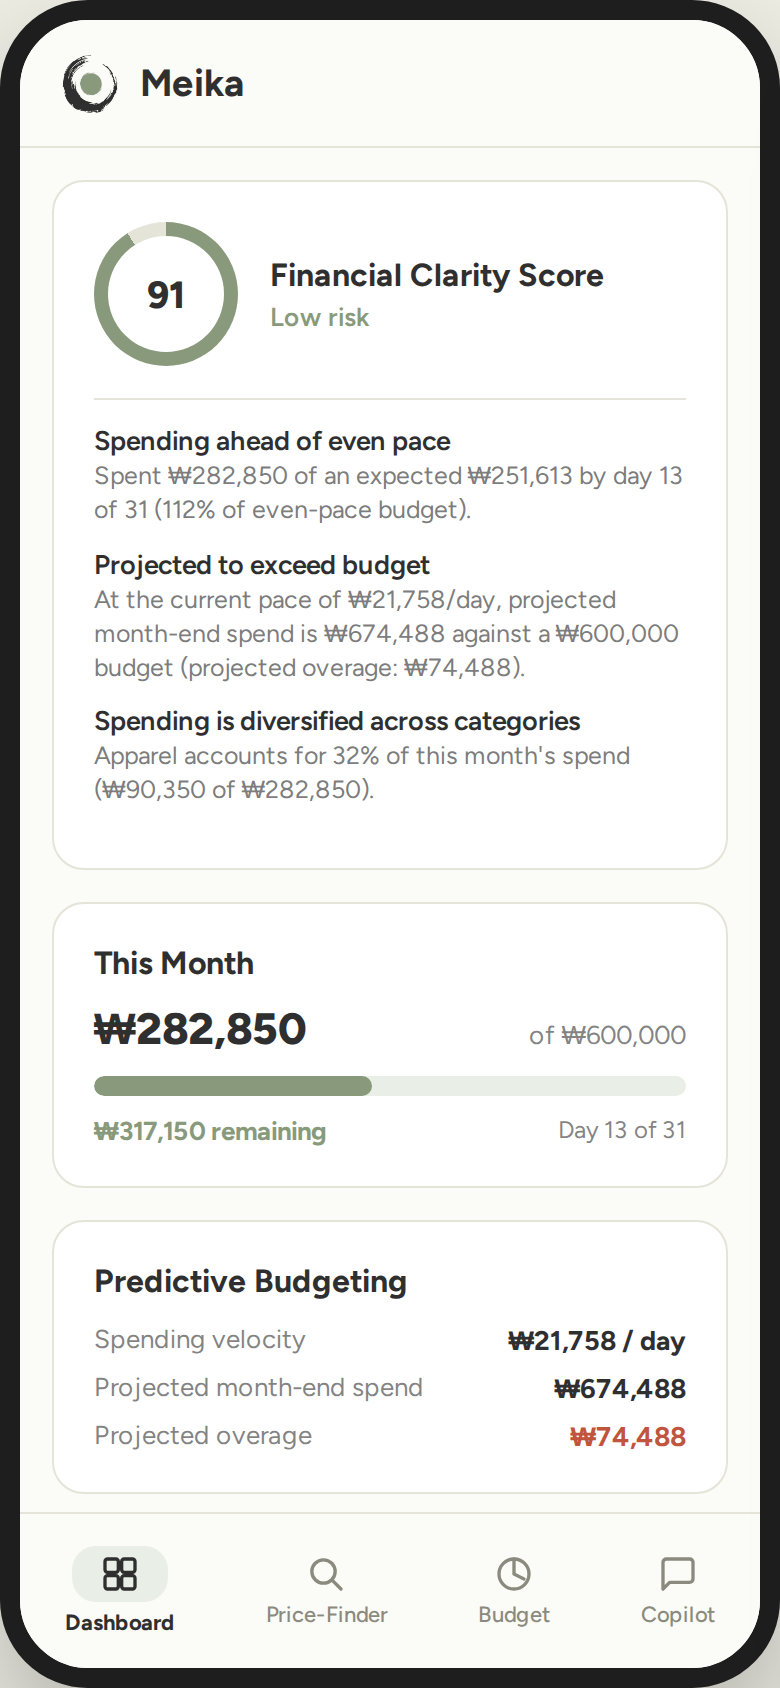
\includegraphics[width=0.47\columnwidth]{fig4a_dashboard.png}
\hfill

\includegraphics[width=0.47\columnwidth]{fig4b_budget.png}
\caption{Flutter client rendering real computed data at the Phase-I review: the dashboard with the Financial Clarity Score and its factor list (left), and the budget screen with the cash-flow outlook and expense history (right).}
\label{fig:screens}
\end{figure}

\subsection{Planned Experimental Evaluation}

The evaluation above establishes functional correctness but not calibration. A fuller evaluation is planned once a larger dataset and a user cohort are available; the intended measures are listed in Table~\ref{tab:futuremetrics}. No results are reported against these measures at this stage, and none should be inferred.

\begin{table}[!t]
\centering
\caption{Planned Evaluation Measures (No Results Reported)}
\label{tab:futuremetrics}
\footnotesize
\renewcommand{\arraystretch}{1.3}
\begin{tabular}{|p{2.8cm}|p{4.7cm}|}
\hline
\textbf{Component} & \textbf{Planned Measure} \\
\hline
Predictive budgeting & MAE, RMSE, and MAPE of projected against realized month-end spend \\
\hline
API performance & Endpoint response time under representative load \\
\hline
Reliability & Automated test pass rate against a provisioned database \\
\hline
Explainability & User comprehension and trust instruments comparing factor-annotated against bare-score presentation \\
\hline
Goal forecasting & Forecast error and goal-attainment prediction accuracy, once implemented \\
\hline
Score calibration & Agreement between the Clarity Score and realized financial outcomes across a diverse user sample \\
\hline
\end{tabular}
\end{table}

\section{Comparative Discussion}

Table~\ref{tab:comparison} positions MEIKA against two reference classes drawn from the reviewed literature: the conventional expense tracker, which records and reports but does not predict, and the black-box AI finance system, which predicts capably but exposes little of its reasoning. The comparison is a statement of design posture, not a claim of measured superiority; the systems in the second column have reported predictive accuracies that MEIKA has not attempted to match and, lacking a trained model, does not directly compete with.

\begin{table}[!t]
\centering
\caption{Comparative Positioning of MEIKA}
\label{tab:comparison}
\footnotesize
\renewcommand{\arraystretch}{1.3}
\begin{tabular}{|p{1.8cm}|p{1.5cm}|p{1.7cm}|p{2.0cm}|}
\hline
\textbf{Feature} & \textbf{Traditional tracker} & \textbf{Black-box AI system} & \textbf{MEIKA} \\
\hline
Expense tracking & Yes & Yes & Yes \\
\hline
Predictive budgeting & Limited & Yes & Yes, deterministic \\
\hline
Explainability & Limited & Limited or absent & Core design constraint \\
\hline
Risk analysis & Reactive & Present but opaque & Proactive, factor-based \\
\hline
Factor traceability & No & Limited & Yes, by construction \\
\hline
Goal forecasting & Limited & Varies & Planned, same constraint \\
\hline
Conversational assistance & Rare & Possible & Implemented, grounded and bounded \\
\hline
Training required & No & Yes & No \\
\hline
Pattern discovery & No & Yes & No (deliberate trade) \\
\hline
\end{tabular}
\end{table}

The final two rows deserve emphasis because they cut against the proposed system. A deterministic scoring engine cannot discover a spending pattern nobody anticipated; a learned model can. MEIKA's design accepts that limitation in exchange for a guarantee the learned model cannot offer -- that every figure shown can be decomposed, reproduced, and contested. The argument advanced here is not that determinism is superior in general, but that for the specific class of outputs on which a user is expected to act financially, an auditable computation is preferable to an unauditable one of comparable or even somewhat greater accuracy. Where pattern discovery is genuinely required, the appropriate extension is a learned component whose outputs are themselves decomposed into named factors before display, rather than an abandonment of the constraint.

\section{Limitations}

The following limitations are stated to bound the claims made above.

\emph{Dataset scale.} The demonstrated evaluation rests on a seeded dataset of seven transactions across six categories. This is adequate to establish that the pipeline functions and inadequate for any inference about behaviour at realistic data volumes.

\emph{Uncalibrated scoring parameters.} The penalty constants in (4) through (6) are design choices, not empirically derived weights. No study has yet established that a score of, say, 70 corresponds to a materially different real-world financial outcome than a score of 60. A structural consequence of the current weights is that the three penalties sum to at most 90, so the attainable score range is effectively $[10, 100]$ rather than the nominal $[0, 100]$; the lower clamp is defensive rather than reachable. Calibration against realized outcomes is required before the score should be treated as a measure rather than an indicator.

\emph{Linearity of the projection.} Month-end projection is a linear extrapolation of mean daily spend. It does not model weekly periodicity, recurring fixed obligations, or known future commitments, and it will systematically misestimate for users whose expenditure is unevenly distributed within the month. The seven-day warm-up guard mitigates the most severe early-month distortions but does not address this.

\emph{Goal forecasting is absent.} It is a stated objective of the project and remains unimplemented.

\emph{The live language-model path is unvalidated.} The Gemini call path is implemented and defensively wrapped, but has not been exercised against a live API key. Its behaviour in production is therefore unverified, and only the deterministic reply path can presently be described as tested.

\emph{Security is an MVP baseline, not an audited posture.} Authentication and rate limiting are implemented, but there is no token revocation or refresh flow, no brute-force lockout beyond the rate limit, no application-layer transport-security enforcement, and no secure client-side token storage. The rate limiter holds state per process and would not function correctly across multiple workers.

\emph{No user study.} No evaluation of whether the factor-based presentation actually improves user comprehension or trust has been conducted. The explainability claim advanced in this paper is structural -- that the explanation faithfully describes the computation -- and structural faithfulness does not by itself establish that users find the explanation useful. This is the most significant gap between what the architecture guarantees and what the project ultimately aims to demonstrate.

\emph{Price-trend reporting is constrained by observation history.} Listings retrieved from live external search are observed once and therefore carry no trend, which the system reports honestly as insufficient data rather than inferring a direction.

\section{Future Work}

Several directions follow directly from the limitations above.

\begin{enumerate}
\item \textbf{Explainable goal forecasting.} Implement goal projection against the observed spend trend, subject to the same construction-time constraint applied to the Clarity Score: a goal projection must emit the factors that produced it or must not be displayed.
\item \textbf{Validation of the language-model path.} Exercise the live Gemini path against a real key, and add adversarial tests confirming that the model cannot introduce a financial figure absent from the grounding context.
\item \textbf{Empirical calibration of the Clarity Score.} Fit the penalty constants against realized financial outcomes across a diverse user sample, and revisit the effective score range noted in Section X.
\item \textbf{Richer projection models.} Extend beyond linear extrapolation to account for intra-month periodicity and known recurring obligations, retaining decomposability into named factors.
\item \textbf{User studies on explainability and trust.} Compare factor-annotated against bare-score presentation on comprehension, trust, and acted-upon recommendations -- the evaluation the structural claim of this paper does not itself supply.
\item \textbf{Larger real and synthetic datasets.} Establish behaviour at realistic transaction volumes and across varied spending profiles.
\item \textbf{Security hardening.} Add token refresh and revocation, secure client-side token storage, brute-force protection, and a shared-store rate limiter suitable for multi-worker deployment.
\item \textbf{Price observation history.} Accumulate longitudinal price observations so that trends can be computed rather than withheld.
\item \textbf{Advanced financial risk modelling.} Introduce additional risk axes -- income volatility, obligation coverage, liquidity buffer -- each admitted only if it can be expressed as a named, auditable factor.
\item \textbf{Bounded learned components.} Where pattern discovery is required, investigate learned models whose outputs are decomposed into named factors before display, extending rather than relaxing the explainability constraint.
\end{enumerate}

\section{Conclusion}

Personal financial management applications are abundant, but most remain systems of record: they report what has happened and leave the user to infer what follows. Where artificial intelligence has been introduced to close that gap, it has largely been introduced as a source of predictions rather than of understanding, and the surveys examined in Section II converge on the resulting difficulty -- that explainability and trust, not raw model capability, are now the binding constraints on useful financial AI.

This paper has presented MEIKA, an explainable AI-based personal financial copilot built on the premise that explainability is an architectural constraint rather than a feature. The system computes predictive budgeting indicators -- spending velocity and month-end projection -- directly from live transaction data, combines them with a category-concentration measure into a deterministic Financial Clarity Score, and emits every contributing factor as a named \texttt{XAIFactor} object carried in the same response as the score itself. Because the penalty and its explanation are constructed in a single operation from the same quantities, the explanation is a restatement of the computation rather than an approximation of it, and a score cannot structurally be displayed without its reasoning. The system is realized as a Flutter client over a layered FastAPI backend and a tenant-isolated PostgreSQL schema, with a language-model layer bounded to rephrasing figures the deterministic layer has already computed.

The contribution is qualified deliberately. At the Phase-I review the prototype demonstrated three tested REST modules producing a Clarity Score of 91 out of 100 with three live factors over a seven-transaction dataset, and the implementation has since been extended with a grounded conversational copilot, a price-comparison module, authentication, and multi-currency display. These establish that the approach is realizable, not that it is calibrated: the scoring parameters remain empirically unvalidated, goal forecasting is not yet implemented, and no user study has tested whether the explanations this architecture guarantees are explanations users actually find useful. Those are the questions the next phase of this work is designed to answer. The claim advanced here is narrower and, the authors suggest, prior to them -- that a financial decision-support system can be built so that no figure reaches the user without its justification, and that this property is worth designing for from the outset rather than retrofitting once trust has already been lost.

% ---------------------------------------------------------------
% REFERENCES -- IEEE numbered style, matches citation keys above
% ---------------------------------------------------------------
\begin{thebibliography}{00}

\bibitem{pathak2010survey}
B. Pathak, ``A Survey of the Comparison Shopping Agent-Based Decision Support Systems,'' \emph{Journal of Electronic Commerce Research}, vol. 11, no. 3, pp. 178--198, 2010.

\bibitem{badiger2026spendai}
R. Badiger, Robin R, T. Moraas, V. G. Naik, and K. A. N, ``Next.js-Powered AI Platform for Smart Expense Tracking, Budgeting and Insights,'' \emph{SSRN Electronic Journal}, Paper ID 6615358, 2026.

\bibitem{deepthi2026aipowered}
Deepthi C G, J. J. Shetty, I. B. Shreeya Jain, Lakshmi C R, and Kiran Kumar D R, ``AI-Powered Finance Management Platform,'' in \emph{Proc. 2026 Int. Conf. on Smart Futuristic Technology (ICSFT)}, Bangalore, India, Jan. 2026, doi: 10.1109/ICSFT.2026.11500666.

\bibitem{kakulapati2026expensetracker}
V. Kakulapati, D. Sumanth, M. Harshitha Reddy, and P. Saisharath, ``AI-Powered Personal Expense Tracker,'' \emph{Grenze International Journal of Engineering and Technology}, Grenze ID: 01.GIJET.12.1.401\_1, 2026.

\bibitem{ganta2025multimodule}
P. Ganta, G. Agarwal, R. Jha, and K. Nagaraj, ``An Intelligent Multi-Module Financial Assistant for Personalized Budgeting, Risk Alerts, and Adaptive Investment Advisory,'' in \emph{Proc. 2025 9th Int. Conf. on Computational System and Information Technology for Sustainable Solutions (CSITSS)}, 2025, doi: 10.1109/CSITSS67709.2025.11294369.

\bibitem{nie2024survey}
Y. Nie, Y. Kong, X. Dong, J. M. Mulvey, H. V. Poor, Q. Wen, and S. Zohren, ``A Survey of Large Language Models for Financial Applications: Progress, Prospects and Challenges,'' \emph{arXiv:2406.11903v1}, Jun. 2024.

\bibitem{khan2025bridging}
A. T. Khan, S. Li, and X. Cao, ``Bridging Finance and AI: A Comprehensive Survey of Large Language Models in Financial System,'' \emph{Digital Finance}, vol. 7, no. 4, 2025, doi: 10.1007/s42521-025-00146-3.

\bibitem{unde2026dashboard}
Unde S. P., A. B. Ghule, R. S. Jaware, S. N. Kanawade, and Y. K. Koli, ``AI-Based Real-Time Personal Finance Dashboard,'' \emph{International Journal of Advanced Research Publications}, vol. 2, no. 6, pp. 1--11, Jun. 2026.

\bibitem{saini2025aipowered}
M. S. Saini, P. Suri, D. Panwar, M. Sharma, S. Bagga, and V. Ahmad, ``AI-Powered Personal Finance Management Applications,'' in \emph{Proc. 2025 World Skills Conf. on Universal Data Analytics and Sciences (WorldSUAS)}, 2025, doi: 10.1109/WorldSUAS66815.2025.11199144.

\bibitem{patil2026nexus}
Patil et al., ``Nexus Finance: AI-Powered Financial Goal Planner for Personalized Budgeting and Investment,'' \emph{International Journal of Research and Innovation in Social Science (IJRISS)}, 2026. [Reference details require verification: full author list, volume, issue, page numbers, and DOI were not available in the supplied source material.]

\end{thebibliography}

% NOTE: References [1]-[7] correspond to the base paper plus the six papers
% shortlisted in the project proposal for discussion with the mentor;
% [8]-[9] (Unde et al., Saini et al.) were added to round out the
% Literature Survey table. [10] (Patil et al.) completes the set of 10
% papers shown in the Review-1 presentation; its bibliographic details are
% INCOMPLETE -- only the title, venue (IJRISS), year, and method were
% recoverable from the presentation. The full author list, volume, issue,
% pages, and DOI MUST be filled in from the original paper before
% submission. Please also verify author names/affiliations for [1]-[9]
% against the original PDFs before final submission.
%
% CITATION ORDER: this bibliography is grouped thematically, not in strict
% order of first appearance ([1] Pathak is first cited in Sec. II-D, and
% [10] Patil in Sec. II-A). Most IEEE venues accept this, but if the target
% venue mandates order-of-appearance numbering, the list must be renumbered
% before submission.

\end{document}
